\onecolumn
\chapter{Auswertung}
\label{ch:auswertung}

\section*{Fehlerrechnung}
Für die statistische Auswertung von $n$ Messwerten $x_i$ werden folgende Größen definiert \cite{errorSkript25}:
\begin{align}
    \bar{x} &= \frac{1}{n} \sum_{i=1}^{n} x_i \vphantom{\sqrt{\sum_i^n}^2} && \text{\textcolor{gray}{Arithmetisches Mittel}} \label{eq:arithmetisches_mittel} \\
    \sigma^2 &= \frac{1}{n-1} \sum_{i=1}^{n} (x_i - \bar{x})^2 \vphantom{\sqrt{\sum_i^n}^2} && \text{\textcolor{gray}{Variation}} \label{eq:variation} \\
    \sigma &= \sqrt{\frac{1}{n-1} \sum_{i=1}^{n} (x_i - \bar{x})^2} \vphantom{\sqrt{\sum_i^n}^2} && \text{\textcolor{gray}{Standardabweichung}} \label{eq:standardabweichung} \\
    \Delta \bar{x} &= \frac{\sigma}{\sqrt{n}} = \sqrt{\frac{1}{n(n-1)} \sum_{i=1}^n(\bar x - x_i)^2} \vphantom{\sqrt{\sum_i^n}^2} && \text{\textcolor{gray}{Fehler des Mittelwerts}} \label{eq:fehler_mittelwert} \\
    \Delta f &= \sqrt{\left(\frac{\partial f}{\partial x} \Delta x\right)^2 + \left(\frac{\partial f}{\partial y} \Delta y\right)^2} \vphantom{\sqrt{\sum_i^n}^2} && \text{\textcolor{gray}{Gauß’sches Fehlerfortpflanzungsgesetz für $f(x,y)$}} \label{eq:gauss_fehlfortpflanzung} \\
    \Delta f &= \sqrt{(\Delta x)^2 + (\Delta y)^2} \vphantom{\sqrt{\sum_i^n}^2} && \text{\textcolor{gray}{Fehler für $f = x + y$}} \label{eq:fehler_summe} \\
    \Delta f &= |a| \Delta x \vphantom{\sqrt{\sum_i^n}^2} && \text{\textcolor{gray}{Fehler für $f = ax$}} \label{eq:fehler_proportional} \\
    \frac{\Delta f}{|f|} &= \sqrt{\left(\frac{\Delta x}{x}\right)^2 + \left(\frac{\Delta y}{y}\right)^2} \vphantom{\sqrt{\sum_i^n}^2} && \text{\textcolor{gray}{relativer Fehler für $f = xy$ oder $f = x/y$}} \label{eq:relativer_fehler} \\
    \sigma &= \frac{|a_{lit} - a_{gem}|}{\sqrt{\Delta a_{lit}^2 + \Delta a_{gem}^2}} \vphantom{\sqrt{\sum_i^n}^2} && \text{\textcolor{gray}{Berechnung der signifikanten Abweichung}} \label{eq:signifikante_abweichung}
\end{align}

\twocolumn

\section{Aufgabe 1: Bestimmung der Faraday-Konstante über Kupferelektroden}
Der Versuchsdurchführung ist zu entnehmen, dass wir zei Kupferelektroden haben. Wir haben die Massen beider vor und nach der Elektrolyse gewogen, um deren Massendiffrenz für die Anode $\delta M{An}$ und die Kathode $\delta M{Ka}$ zu bestimmen.
Wir führen die Ergebnisse der \hyperref[Protokoll]{ersten Tabelle des Protokoll} auf:
\begin{table}
    \begin{tabular}{c | c | c}
        \toprule
        Masse & Anode$^+$ & Katode$^-$\\
        \hline
        Zuvor  [g] & 87,3815 & 90,6317 \\
        Dannach [g] & 86,5189 & 91,4648 \\
        \midrule
        $\delta m \, [g]$ & -0,8626 & 0,8331\\
        \bottomrule
    \end{tabular}
    \label{tab:p_1}
    \caption{Gemessene Werte, bei einem Strom $I$ von $1,01A$ und einer Zeit von 41:28 (mm:ss).}
\end{table}

Dabei gehen wir für die folgenden Fehlerrechnungen mit einer Ungenauigkeit der Waage von $0,001g$ aus, und vom Netzteil von $(2\% \pm 0,02)A$.
Eine Ungenaugkeit der Zeit ist etwas merkwürdig, da die Stoppzeit selbst nicht die Zeit zwischen Herausnehmen der Kupferplatten, deren Trocknung und das Wiegen berücksichtigt.
Dennoch wurde zu diesem Zeitpunkt der Strom ausgestellt und es wird eine Ungenauigkeit der Menschlichen Reaktionszeit von $0,300s$ angenommen. Dies hat zwar keine große Auswirkung,
wird jedoch berücksichtigt.

Die chemischen Gleichungen sind bereits in der \hyperref[sc:Massenmessung]{Einleitung (\ref*{sc:Massenmessung})} beschrieben. Daher gehen wir gleich zur Berechnung über.

Dafür stellen wir \hyperref[eq:first_faraday]{Gleichung \ref*{eq:first_faraday}} um zu
\begin{equation}
    F = \frac{Q \cdot M_{Mol}}{z \cdot m}
\end{equation}
und werden ihre einzelnen Komponenten nun bestimmen.

Wir haben dabei eine Gesamtladung $Q$ nach \hyperref[eq:ladung]{Gleichung \ref*{eq:ladung}} von:
\begin{equation}
    Q = 2512,88 C.
\end{equation}
Wobei wir für $I = 1,01A$ eingesetzt haben und für $t = 2488s$.

Die Ungenauigkeit der Ladung wird via \hyperref[eq:gauss_fehlfortpflanzung]{Gauß'scher Fehlerfortpflanzung (\ref*{eq:gauss_fehlfortpflanzung})} bestimmt:
\begin{equation}
    \Delta Q = \sqrt{\left( \frac{\Delta I}{I} \right)^2 + \left( \frac{\Delta t}{t} \right)^2} \cdot Q.
\end{equation}

Damit kommen wir auf eine Ladung von 
\begin{equation}
    \underline{Q = (2513 \pm 100)C}.
\end{equation}

Die Werte für die Massen entnehmen wir der \hyperref[tab:p_1]{Tabelle \ref*{tab:p_1}}. Und kommen auf Massendifferenz von:
\begin{equation}
    \underline{
        \delta m_{An} = (-0,8626 \pm 0,001) g
    }
\end{equation}

\begin{equation}
    \underline{
        \delta m_{Ka} = (0,8331 \pm 0,001) g
    }
\end{equation}
Dabei heiß eine negative Massendifferenz, Massenverlust, während der positive Wert eine Massenaufnahme bedeutet. Die Kathode wurde also schwerer. Wir nehmen zur berechnen der Faraday-Konstante die Betäge, der Massendifferenzen.

Die Molare Masse ist einem Periodensystem \cite{CuMol} zu entnehmen, und beträgt $M_{cu} = 63,546 \frac{g}{mol}$. Die Wertigkeit ist der Reaktionsgleichungen zu entnehmen und entspricht $2$, da unsere Kupferionen zwei-Fach positiv geladen sind.

Damit kommen wir auf zwei Faraday-Konstanten, für jede Elektrode:
\begin{equation}
    \underline{F_{Ka} = 92559,397} \frac{C}{mol}
\end{equation}

\begin{equation}
    \underline{F_{An} = 95836,918} \frac{C}{mol}.
\end{equation}

Nun fehlt nur noch die Bestimmung der Ungenauigkeit. Dafür nutzen wir \hyperref[eq:gauss_fehlfortpflanzung]{Gauß'sche Fehlerfortpflanzung} und kommen damit auf:
\begin{equation}
    \Delta F = \sqrt{\left(\frac{\Delta Q}{Q}\right)^2 + \left(\frac{\Delta m}{m}\right)^2}
\end{equation}

Dabei ist die Wertigkeit $z$ ohne Frage fehlerfrei, jedoch gäbe es theoretisch eine Ungenauigkeit der Molarenmasse, einen sicheren Wert konnte ich jedoch nicht finden,
alle Werte die man findne konnte, haben das Ergebniss aber ohne hin nicht verändert.

Die Fehler berufen sich auf:
\begin{equation}
    \underline{\Delta F_{Ka} = 3684,898} \frac{C}{mol},
\end{equation}

\begin{equation}
    \underline{\Delta F_{An} = 3815,264} \frac{C}{mol}
\end{equation}


Setzt man nun alles zusammen, und runden nach den signifikanten Stellen, so kommen wir auf Ergebnisse von:
\begin{equation}
    \boxed{
        F_{Ka} = (93000 \pm 4000) \frac{C}{mol}
    }
\end{equation}
und
\begin{equation}
    \boxed{
        F_{An} = (96000 \pm 4000) \frac{C}{mol}.
    }
\end{equation}

Jetzt ist natürlich die Frage, ob die Werte untereinander statistisch signifikant sind. Dies wollen wir berechnen und kommen auf:
\begin{equation}
    \frac{\left| F_{Ka} - F_{An} \right|}{\sqrt{(\Delta F_{Ka})^2 + (\Delta F_{An})^2} } = 0,53\sigma
\end{equation}

Die Werte decken sich also Statistisch gegenseitig. 
Als letztes in diesem Aufgabenteil wollen wir den Vergleich zu den Literaturwerten ziehen und kommen dabei auf:

\begin{equation}
    \frac{\left| F_{Ka} - F_{lit} \right|}{\sqrt{(\Delta F_{Ka})^2 + (\Delta F_{lit})^2} } = 0,87\sigma
\end{equation}
und
\begin{equation}
    \frac{\left| F_{lit} - F_{An} \right|}{\sqrt{(\Delta F_{lit})^2 + (\Delta F_{An})^2} } = 0,12\sigma.
\end{equation}
Die Werte decken sich also mit dem Literaturwert.



\section{Aufgabe 2: Bestimmung der Faraday-Konstante aus der Elektrolise von Wasser}
Die chemischen Gleichungen sind bereits in der \hyperref[sc:faraday_vol]{Einleitung (\ref*{sc:faraday_vol})} beschrieben. Daher gehen wir gleich zur Berechnung über.


Wir führen die Ergebnisse der \hyperref[Protokoll]{zweiten Tabelle des Protokoll} auf:
\begin{table}
    \centering
    \begin{tabular}{c | c | c}
        \toprule
        Säule & Startvolumen [ml] & Endvolumen [ml] \\
        \hline
        Sauerstoff & $0,50 \pm 0,10$ & $21,60 \pm 0,1$ \\
        Wasserstoff & $5,20 \pm 0,10$ & $43,20 \pm 0,10$ \\
        \bottomrule
    \end{tabular}
    \caption{Start- und Endvolumina der zwei Säulen.}
\end{table}

Wichtig zu verstehen ist, dass der angegebene Volumenswert nicht das Volumen der Flüssigkeit ist, sondern das Volumen über der Flüssigkeit. 
Das Startvolumen wurde nach 30 Sekunden Elektrolyse bestimmt. Das Endvolumen, als es möglichst weit unten war, damit die Differenz möglichst groß wird, da so der Ablesefehler prozentual kleiner wird.
Die verdampften Volumina sind dabei:
\begin{align}
    V_{O_2} = (21,10 \pm 0,10) ml, \\
    V_{H_2} = (38,00 \pm 0,10) ml.
\end{align}

Als nächstes brauchen wir die jeweiligen molaren Volumina $V_{Mol}$, um aus deren Verhältnissen nach \hyperref[eq:stoffmenge]{Gleichung \ref*{eq:stoffmenge}} die Stoffmenge zu bestimmen. 
Dafür nutzen wir \hyperref[eq:molvolumen]{Gleichung \ref*{eq:molvolumen}} und \hyperref[eq:druck]{Gleichung \ref*{eq:druck}}.

Wir benutzen für den Druck $p_0 = 1013,25 hPa$, und für die Temperatur $273,15K$, da hier das ideale Gas Gesetz das Volumen $V_0^{Mol} = 22,414 \frac{L}{mol}$ ergibt.
Nun brauchen wir noch das Verhältnis der Raumtemperatur $T = (24,0 \pm 1,0)^\circ C$ über den druck $p$. 

Den Druck $P_{H_2O}^D$ kann man via \hyperref[tab:wasser_druck]{Tabelle \ref*{tab:wasser_druck}} bestimmen, wo bei wir eine Wassertemperatur von $T_W = (26,0 \pm 1,0)^\circ C$ haben. Somit ist unser Druck:
\begin{equation}
    p_{H_2O}^D = 25,76 Torr \, \hat= \, 34,3 hPa.
\end{equation}

Mit einem Gemessenen Luftdruck von $(p = 1000,0 \pm 0,5) \, hPa$ kommt man somit afu ein molares Volumen von
\begin{equation}
    V_{Mol} = 25,580  \, \frac{L}{mol}.
\end{equation}

Dabei haben wir den Druck zu $p = 969,13 hPa$ berechnet.

Als nächstes müssen wir die Ungenauigkeit über die \hyperref[eq:gauss_fehlfortpflanzung]{Gauß'scher Fehlerfortpflanzung (\ref*{eq:gauss_fehlfortpflanzung})} bestimmen. 

Die Ungenauigkeit des berechneten Druckes ergibt sich zu
\begin{equation}
    \Delta p = \sqrt{(\Delta p_L)^2 + (0,9 \cdot \Delta p_{H_2O}^D)^2}.
\end{equation}

Wir haben dabei die Ungenauigkeit des Luftdruckes $\Delta p_L = 0,5 hPa$. Die des Wasserdruckes ergibt sich über die Temperaturungenauigkeit von $\Delta T_{H_2O} =1^\circ C$.
Die Ungenauigkeit liegt daher bei $\Delta p_{H_2O}^D = 1,75 Torr$, dies wiederrum erntspricht $2,3 hPa$. Dies wurde bestimmt, in dem das Maximum der Differenzen mit den zwei umliegenden Werten gezogen wurde.

Setzen wir unsere Ungenauigkeiten ein, kommen wir auf einen Wert von
\begin{equation}
    \Delta p = 2,130 hPa.
\end{equation}

Damit lässt sich die Ungenauigkeit des molaren Volumens zu 
\begin{equation}
    \Delta V_{Mol} = \frac{p_0 \cdot V_{0,Mol}}{T_0} \sqrt{\left(\frac{\Delta T}{p}\right)^2 + \left(\frac{T \cdot \Delta p}{p^2}\right)^2}
\end{equation}  
berechen.

Über diese können wir nun unser finales molares Volumen bestimmen:
\begin{equation}
\boxed{
    V_{Mol} = (25,580 \pm 0,090)\, \frac{L}{mol}.
}
\end{equation}

Somit kommen wir auf eine Stoffmenge des Wasserstoffes von
\begin{equation}
    n_{H_2} = 1,5 mol, 
\end{equation}
und einer Stoffmenge des Sauerstoffes von 
\begin{equation}
    n_{O_2} = 0,8 mol.
\end{equation}

Den Reaktionsgleichungen (\ref*{eq:h2_kathode}, \ref*{eq:o2_anode}) sind die Wertigkeiten $z_{H_2} = 2$ und $z_{O_2} = 4$ zu entnehmen.

Der letzte zu bestimmende Wert ist die Ladung $Q$.



\section{Aufgabe 3: Elektrolyse in einer Brennstoffzelle}

In dieser Aufgabe wird das Funktionsprinzip einer PEM-Brennstoffzelle untersucht, die die umgekehrte Reaktion der Elektrolyse nutzt. Der Versuch liefert qualitative Beobachtungen über die Umwandlung chemischer Energie in elektrische Energie.

\begin{enumerate}
    \item \textbf{Anode: Spaltung von Wasserstoff}\\
    Wasserstoff (H$_2$) wird an der Anode in Protonen (H$^+$) und Elektronen gespalten:
    \begin{equation*}
        2 \mathrm{H_2 \rightarrow 4 H^+ + 4 e^-} \quad (\text{\hyperref[eq:h2_anode]{Gleichung \ref*{eq:h2_anode}}})
    \end{equation*}
    Die Protonen passieren die protonenleitfähige Membran zur Kathode, während die Elektronen über einen externen Stromkreis fließen.
    
    \item \textbf{Kathode: Reaktion zu Wasser}\\
    An der Kathode reagieren Protonen, Elektronen und Sauerstoff zu Wasser:
    \begin{equation*}
        4 \mathrm{H^+ + 4 e^- + O_2 \rightarrow 2 H_2O} \quad (\text{\hyperref[eq:h2o_kathode]{Gleichung \ref*{eq:h2o_kathode}}})
    \end{equation*}
    Dabei entsteht Wasser, das als Kondensat sichtbar sein kann.

    \item \textbf{Gasverbrauch}\\
    Mit Beginn der Reaktion nimmt die Menge an Wasserstoff und Sauerstoff an den Elektroden ab, was die Umwandlung der chemischen Energie in elektrische Energie sichtbar macht.

    \item \textbf{Elektrischer Stromfluss}\\
    Ein angeschlossener Verbraucher kann die elektrische Energie abnehmen. Der Stromfluss zeigt die Nutzung der freiwerdenden Energie an.

    \item \textbf{Interpretation}\\
    Die Beobachtungen bestätigen die Umkehrung der Elektrolyse: Energie, die zuvor zur Zerlegung von Wasser benötigt wurde, wird nun durch die kontrollierte Reaktion von H$_2$ und O$_2$ freigesetzt und kann direkt als elektrische Energie genutzt werden.
\end{enumerate}

\section{Zusatz: Kupferoxidation an der Luft/unterm Föhn}
Wir wollen hier nun die Fehlerrechnung noch mal ein wenig vertiefen und eine weitere Fehlerquelle betracheten und ihren Einfluss untersuchen. Wir wollen schauen, wie viel Kupfer in der Zeit nach der Elektrolise und bis zum Wiegen Oxidieren.
Der Grund dafür ist, dass die zu wiegende Kathode nach der Elektrolyse kein konstantes Gewicht eingenommen hat, sondern das Gewicht über wenige Minuten um knapp $1mg$ anwuchst, ohne aufzuhören.
Die gestellte These hier ist, dass dies insbesondere durch den Einfluss des Föhns passiert, denn dieser hat die Kupferplatte erhitzt. Und bei Oxidationsvorgängen ist eine thermische Energiezufur equivalent zu einer Beschleunigung der Reaktion.
Die Platte hat sich dabei natürlcih nicht auf enorme Temperaturen erhitzt, aber es dürfte schon ausreichen, wenn die Oberfläche sich erhitzt, da sowieso nur an der Oberfläche die Oxidation stattfindet. In der Studie \cite{KupferStudie}
wurde mit Temperaturen im $60^\circ C$ gearbeitet. Für diese Untersuchung nehme ich die Werte als möglich an und als Basis der folgenden Untersuchung.

Wichtig ist hie rnatürlich zu erwähnen, dass die Rechnung kaum ernstzunehmen ist, die Werte und Überlegungen sind für sinnvolle Angaben kaum nutzbar und sollen erstmal die grundsetzliche Frage klären, ob die Oxidation an der Luft und das Fühnen einen signifikaten Einfluss haben könnten.

Dafür müssen wir einige Werte schätzen, dessen Messung leider nicht stattfund.
\begin{align}
    A_{Cu} &\approx (25 \pm 5)cm^2 \\
    t &\approx (300\pm100)s
\end{align}
Dabei ist $A_{Cu}$ die Kupferfläche, die Reagiert und $t$ die Zeit, in der die Reaktion stattfindet.

Wir leiten dabei graphisch die Massengewichstzunahme $\delta m$ her. Dafür haben wir \hyperref[eq:stud_log]{Gleichung (\ref*{eq:stud_log})} in Python geplottet. Der Code fafür ist auf meinen GitHub \cite{githubPAP1}. 
Dabei sind vier \hyperref[fig:log_3]{Graphen \ref*{fig:log_3}} geplottet. Wir konzentrieren uns dabei auf die logarithmischskalierten Graphen und fabei auf den blauen (unterster) und den roten (obester) und suchen graphisch nach unserer Massenzunahme. 

Dabei kommen wir auf Werte von:
\begin{align}
    \delta m_{min} &= (1,11 \pm 0,06)\frac{\mu g}{cm^2} \\
    \delta m_{max} &= (1,86 \pm 0,09)\frac{\mu g}{cm^2}
\end{align}

Dabei haben wir daruf geachtet, nur im Bereich zu bleiben, der in der \hyperref[fig:stud_2]{Abbildung \ref*{fig:stud_2}} auch rot eingezeichnet ist zu bleiben.

Die entstandene Masse sollte nun ziemlich leicht zu berechnen sein. Somit ergibt sich für die minimal Abschätzung
\begin{equation}
    m_{min} = 1,11 \frac{\mu g}{cm^2} \cdot 25cm^2 = 27,75 \mu g 
\end{equation}
udn für die Maximalabschätzung
\begin{equation}
    m_{max} = 1,86 \frac{\mu g}{cm^2} \cdot 25cm^2 = 46,5 \mu g.
\end{equation}

Wir wollen natürlich noch die Ungenauigkeit bestimmen. Daher \hyperref[eq:gauss_fehlfortpflanzung]{Gauß'sche Fehlerfortpflanzung}:
\begin{equation}
    \Delta m = \sqrt{\left(\frac{\Delta \delta m}{\delta m} \right)^2 + \left(\frac{\Delta A_{Cu}}{A_{Cu}} \right)^2}
\end{equation}

Damit kommen wir auf Massen von 
\begin{equation}
    \boxed{\delta m_{min} = (27,750 \pm 0,207) \mu g}
\end{equation}
und
\begin{equation}
    \boxed{\delta m_{max} = (46,500 \pm 0,206 ) \mu g}.
\end{equation}

Das heißt, nach 5 Minuten sollen wir einen Massenanstieg der Kupferplatte von zwischen (gerundet) $0,00003g$ und $0,00005g$ erwarten.
Die ist nicht koheränt mit der Beobachtung an der Waage, hier hätten wir eher den Wert um einen Faktor 10 größer vermutet.
Also auch die Oxidationsfläche auf vorder und Rückseite zu berufen hilft nicht, was sowieso sinnvoll gewesen wäre, aber ignoriert wurde, da eine höhre wahrscheinlichkeit vermutet wurde, dass das noch nicht fest angesetzte Kupfer ggf. reagiert.
Dennoch sind die Werte unglaublich nah an den Schwankungen, die zu beobachten waren, also gut möglich, dass diese doch einen Einfluss hatten.Vielleicht wurde auch die verstrichene Zeit unterschätzt, wobei dies wieder kaum einen unterschied gemacht hätte. Am plausielsten wäre, wenn der Föhn die Kupferplatte auf sogar über $60^\circ C$ erhitzt hätte, dies könnte einen signifikanten unterschied machen.
Trozdessen wäre es nicht zielführend, diese Werte noch als Ungenauigkeit in die Rechnung mit aufzunehmen, da diese sowieso unter der Messgenauigkeit der Waage liegen, dessen Fehler um einen Faktor 100 größer ist.

\onecolumn
\begin{figure}
    \includegraphics[width=\textwidth, page=2]{img/21/Plots_oxi-eingezeichnet.pdf}
    \caption{Entstandene Graphen aus der Gleichung, die in der Studie gegeben ist, mit verschiedenen $k_log$ konstanten. Blau soll dabei die Minimalabschätzung und rot die Maximalabschätzung werden.}
    \label{fig:log_gezeichnet}
\end{figure}
\twocolumn